\documentclass[wide,a4paper,titlepage,12pt] {article}
\usepackage{polski}
\usepackage[utf8]{inputenc}
\usepackage{listings}
\usepackage{slashbox}
\usepackage[table]{xcolor}
\usepackage{graphicx,pdflscape}
\usepackage{placeins}
\usepackage{slashbox}
\usepackage{longtable}


\title{Projektowanie efektywnych algorytmów}
\author{Tymon Tobolski (181037)\\ Jacek Wieczorek (181043)}

% Title page layout (fold)
\makeatletter
\renewcommand{\maketitle}{
\begin{titlepage}
  \begin{center}
    \vspace*{3cm}
    \LARGE \@title \par
    \vspace{2cm}
    \textit{\small Autor:}\par
    \normalsize \@author\par \normalsize
    \vspace{3cm}
    \textit{\small Prowadzący:}\par
   Prof. dr hab. inż Adam Janiak \par
    \vspace{2cm}
    Wydział Elektroniki\\ III rok\\ Cz TN 13.15 - 15.00\par
    \vspace{4cm}
    \small \@date
  \end{center}
\end{titlepage}
}
\makeatother

\begin{document}
\maketitle

\section{Cel projektu}
\paragraph{}
  Celem projektu jest zaimplementowanie i przetestowanie metaheurystycznego algorytmu genetycznego dla problemu szeregowania zadań na jednym procesorze przy kryterium minimalizacji ważonej sumy opóźnień zadań.

\section{Opis problemu}
{\bf Jednoprocesorowy problem szeregowania zadań przy kryterium
minimalizacji ważonej sumy opóźnień zadań.}

\paragraph{}
Danych jest $n$ zadań (o numerach od 1 do $n$), które mają być wykonane bez przerwań przez pojedynczy procesor, mogący wykonywać co najwyżej jedno zadanie jednocześnie.
Każde zadanie j jest dostępne do wykonania w chwili zero, do wykonania wymaga $p_{j} > 0$ jednostek czasu oraz ma określoną wagę (priorytet) $w_{j} > 0$ i oczekiwany termin zakończenia
wykonywania $d_{j} > 0$. Zadanie $j$ jest spóźnione, jeżeli zakończy się wykonywać po swoim terminie $d_{j}$, a miarą tego opóźnienia jest wielkość $T_{j} = max(0, C_{j} - d_{j} )$, gdzie $C_{j}$ jest terminem zakończenia
wykonywania zadania $j$. Problem polega na znalezieniu takiej kolejności wykonywania zadań (permutacji) aby zminimalizować kryterium $TWT = \Sigma_{j=1}^{n} w_{j} T_{j}$.

\section{Opis algorytmu}
\paragraph{}
Przebieg algorytmu :
\lstset{ %
    language=java,                % choose the language of the code
    basicstyle=\scriptsize,       % the size of the fonts that are used for the code
    numbers=left,                   % where to put the line-numbers
    numberstyle=\scriptsize,      % the size of the fonts that are used for the line-numbers
    stepnumber=10,                   % the step between two line-numbers. If it's 1 each line
                                    % will be numbered
    numbersep=9pt,                  % how far the line-numbers are from the code
    % backgroundcolor=\color{white},  % choose the background color. You must add \usepackage{color}
    showspaces=false,               % show spaces adding particular underscores
    showstringspaces=false,         % underline spaces within strings
    showtabs=false,                 % show tabs within strings adding particular underscores
    % frame=single,                 % adds a frame around the code
    % tabsize=2,                  % sets default tabsize to 2 spaces
    % captionpos=b,                   % sets the caption-position to bottom
    breaklines=true,                % sets automatic line breaking
    % breakatwhitespace=false,        % sets if automatic breaks should only happen at whitespace
    % title=\lstname,                 % show the filename of files included with \lstinputlisting;
                                    % also try caption instead of title
    % escapeinside={\%*}{*)},         % if you want to add a comment within your code
    % morekeywords={*,...}            % if you want to add more keywords to the set
    }
    \lstinputlisting{code/pseudokod.txt}
    \paragraph{}
    gdzie :
    \begin{itemize}
        \item F - funkcja kosztu/celu
        \item M - prawdopodobieństwo mutacji

    \end{itemize}

\section{Implementacja}
\paragraph{}
Jezykiem implementacji algorytmu jest $Scala$ w wersji $2.9.1$ działająca na $JVM$.
\paragraph{}
\lstset{ %
    language=java,                % choose the language of the code
    basicstyle=\scriptsize,       % the size of the fonts that are used for the code
    numbers=left,                   % where to put the line-numbers
    numberstyle=\scriptsize,      % the size of the fonts that are used for the line-numbers
    stepnumber=10,                   % the step between two line-numbers. If it's 1 each line
                                    % will be numbered
    numbersep=9pt,                  % how far the line-numbers are from the code
    % backgroundcolor=\color{white},  % choose the background color. You must add \usepackage{color}
    showspaces=false,               % show spaces adding particular underscores
    showstringspaces=false,         % underline spaces within strings
    showtabs=false,                 % show tabs within strings adding particular underscores
    % frame=single,                 % adds a frame around the code
    % tabsize=2,                  % sets default tabsize to 2 spaces
    % captionpos=b,                   % sets the caption-position to bottom
    breaklines=true,                % sets automatic line breaking
    % breakatwhitespace=false,        % sets if automatic breaks should only happen at whitespace
    % title=\lstname,                 % show the filename of files included with \lstinputlisting;
                                    % also try caption instead of title
    % escapeinside={\%*}{*)},         % if you want to add a comment within your code
    % morekeywords={*,...}            % if you want to add more keywords to the set
    }
    \lstinputlisting{code/gen.scala}

\section{Testy}
\paragraph{}
Test algorytmu tabu search przeprowadzony został dla trzech zestawów testów o różnej ilośći zadań, każdy składający się ze 125 instancji.

\paragraph{}
Jako wyniki testów przedstawiamy średni czas liczenia wszystkich instancji dla danego rozmiaru problemu - $\bar{t}$, a także średni błąd wzgledny  rozwiązań dla każdej instancji - $\bar{x}$. Według wzoru : \\
\begin{equation}
    \bar{t} = \frac{\Sigma_{j=1}^{m}\frac{\Sigma_{i=1}^{z}t_{i}}{z}}{m}
\end{equation}
\begin{equation}
    \bar{x} = \frac{\Sigma_{j=1}^{m}\frac{\Sigma_{i=1}^{z}x_{i}}{z}}{m}
\end{equation}
gdzie : \\
\begin{itemize}
  \item $z$ - ilość rozwiązań w instancji
  \item $m$ - ilość instancji danego problemu
\end{itemize}

\newpage
\subsection{Średnia różnica dla zmiennego \textit{k} i stałego \textit{n = 100}}
\paragraph{}
\begin{center}
    \begin{longtable}{|c|c|c|c|c|}
        \hline
        \backslashbox{$I$}{$k$} & 50 & 100 & 150 & 200 \\ \hline
        40 & 108.04 & 57.86 & 38.76 & 26.19 \\ \hline
        50 & 928.76 & 212.16 & 92.89 & 69.96 \\ \hline
        100 & 2,535.24 & 1,682.69 & 1,133.71 & 859.94 \\ \hline
        \caption{Diff, n=100}
     \end{longtable}
\end{center}

\begin{figure}[htbp]
  \begin{center}
         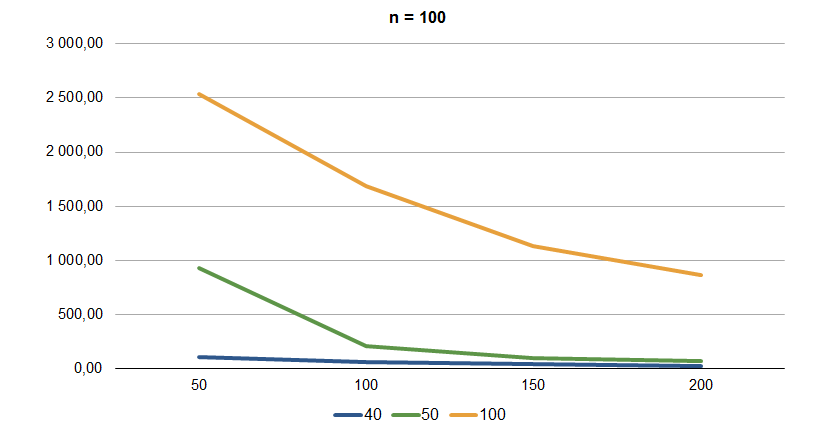
\includegraphics[scale = 0.7]{img/GA_diff_100.PNG}
         \caption{Diff, n=100}
  \end{center}
\end{figure}

\newpage
\subsection{Średnia różnica dla zmiennego \textit{k} i stałego \textit{n = 1000}}
\paragraph{}
\begin{center}
    \begin{longtable}{|c|c|c|c|c|}
        \hline
        \backslashbox{$I$}{$k$} & 50 & 100 & 150 & 200\\ \hline
        40 & 10.99 & 2.59 & 2.53 & 1.44\\ \hline
        50 & 14.33 & 9.17 & 2.14 & 48.89\\ \hline
        100 & 378.84 & 87.50 & 46.63 & 39.68\\
        \hline
        \caption{Diff, n=1000}
    \end{longtable}
\end{center}

\begin{figure}[htbp]
  \begin{center}
         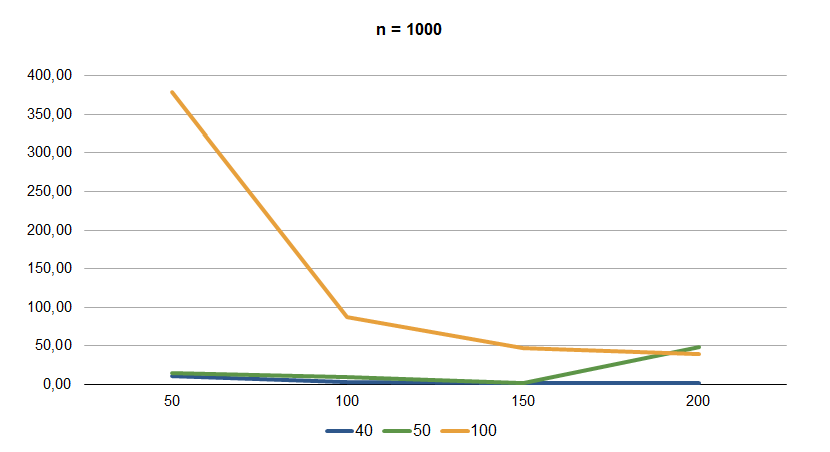
\includegraphics[scale = 0.7]{img/GA_diff_1000.PNG}
         \caption{Diff, n=1000}
  \end{center}
\end{figure}

\newpage
\subsection{Średnia czas rozwiązywania dla zmiennego \textit{k} i stałego \textit{n = 100}}
\begin{center}
    \begin{longtable}{|c|c|c|c|}
        \hline
        \backslashbox{$k$}{$I$} & 40 & 50 & 100\\ \hline
            50 & 136.45 & 219.75 & 497.38\\ \hline
            100 & 261.98 & 391.01 & 918.89\\ \hline
            150 & 409.4 & 598.76 & 1394.21\\ \hline
            200 & 572.62 & 908.32 & 1847.48\\ \hline

        \caption{Time, n=100}
    \end{longtable}
\end{center}

\begin{figure}[htbp]
  \begin{center}
         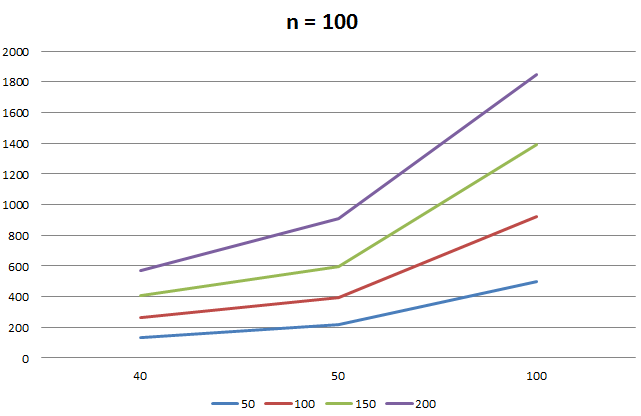
\includegraphics[scale = 0.7]{img/GA_n_100.PNG}
         \caption{Time, n=100}
  \end{center}
\end{figure}


\newpage
\subsection{Średnia czas rozwiązywania dla zmiennego \textit{k} i stałego \textit{n = 1000}}
\begin{center}
    \begin{longtable}{|c|c|c|c|}
        \hline
        \backslashbox{$k$}{$I$} & 40 & 50 & 100\\ \hline
            50 & 1285.72 & 1904.94 & 4428.43\\ \hline
            100 & 2492.99 & 3706.92 & 9026.62\\ \hline
            150 & 3713.95 & 5595.2 & 13981.76\\ \hline
            200 & 4954.24 & 7452.48 & 18717\\
        \hline
        \caption{Time, n=1000}
    \end{longtable}
    
\end{center}

\begin{figure}[htbp]
  \begin{center}
         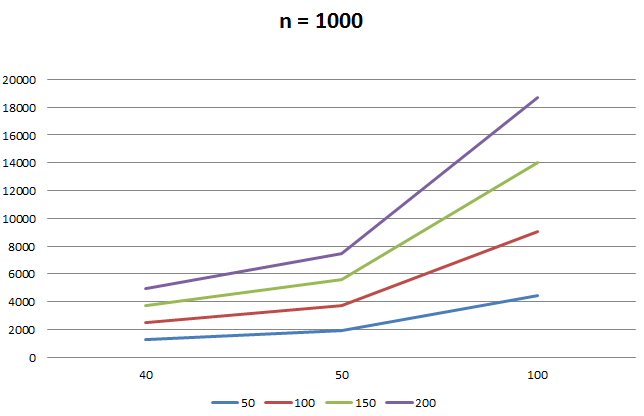
\includegraphics[scale = 0.7]{img/GA_n_1000.PNG}
         \caption{Time, n=1000}
  \end{center}
\end{figure}


\newpage

\section{Wnioski}
\paragraph{}
TODO


\newpage
\section{Porównanie}
\paragraph{} % (fold)
\label{par:}
\subsection{Porównanie średniego czasu algorytmów}
\begin{center}
    \begin{longtable}{|c|c|c|c|}
        \hline
        Alg & 40 & 50 & 100 \\ \hline
        G(k=50, n=100) & 136,45 & 219,75 & 497,38\\ \hline
        G(k=100, n=100)& 261,98 & 391,01 & 918,89\\ \hline
        G(k=150, n=100)& 409,4 &  598,76 & 1394,21\\ \hline
        G(k=200, n=100)& 572,62 & 908,32 & 1847,48\\ \hline
        G(k=50, n=1000)& 1285,72& 1904,94& 4428,43\\ \hline
        G(k=100, n=1000)  &  2492,99 &3706,92& 9026,62\\ \hline
        G(k=150, n=1000)   & 3713,95 &5595,2  &13981,76\\ \hline
        G(k=200, n=1000)   & 4954,24& 7452,48& 18717\\ \hline
        TS(n=10, k=4, t=7) & 23,11 &  46,81 &  333,83\\ \hline
        TS(n=10, k=5, t=7) & 25,96 &  50,96 &  368,84\\ \hline
        TS(n=10, k=6, t=7) & 26,23 &  39,14 &  327,85\\ \hline
        TS(n=10, k=7, t=7) & 19,42  & 38,48  & 314,94\\ \hline
        TS(n=100, k=4, t=7)& 188,06 & 378,68 & 3028,87\\ \hline
        TS(n=100, k=5, t=7)& 208,98 & 375,12 & 3009,74\\ \hline
        TS(n=100, k=6, t=7)& 206,57 & 382,79 & 3004,64\\ \hline
        TS(n=100, k=7, t=7) &185,13  &387,76 & 3003,1\\ \hline
        SA(0,990000)  &  1,89  &  2,01 &   3,09\\ \hline
        SA(0,999000)  &  15,88 &  18,74 &  30,36\\ \hline
        SA(0,999900)  &  167,36 & 189,63 & 305,09\\ \hline
                \caption{Średni czas}
    \end{longtable}
    
\end{center}

\begin{landscape}
\begin{figure}[htbp]
  \begin{center}
         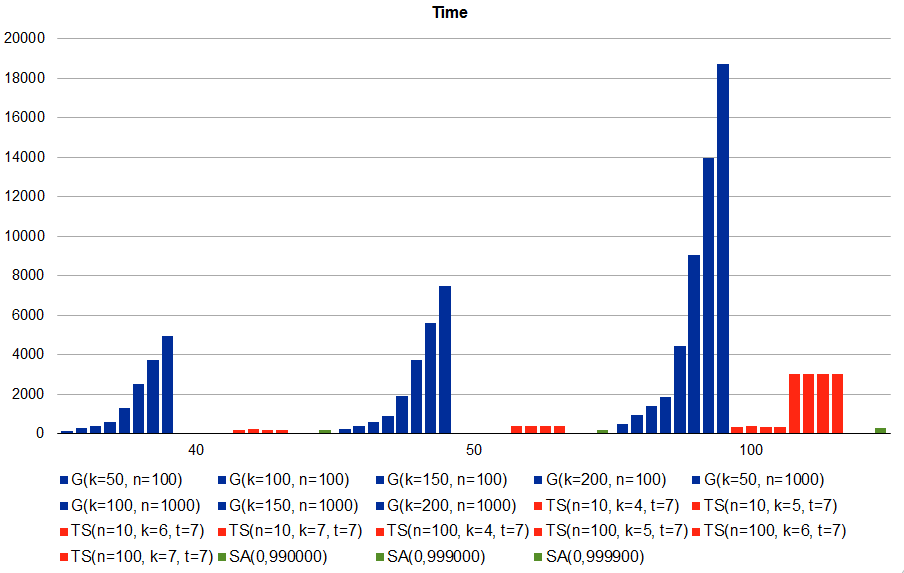
\includegraphics[scale = 1.0]{img/timeAll.PNG}
         \caption{Średni czas}
  \end{center}
\end{figure}
\end{landscape}
\end{document}



